\chapter{System Model}
Cuttlefish, as mentioned earlier, is a 3D printing pipeline which performs the preprocessing of the 3D model and conversion of the virtual design to a form understood by the print machine. The virtual blueprint of the object i.e. the digital model of the object to be printed is created using a designing software. Cuttlefish allows for numerous file formats like STL, Obj, Ply, Wrl as input giving the designer the flexibility to use a designing software of his choice. The whole pipeline has a streaming architecture, which means that the input can processed in smaller parts so as to generate the output sooner thus letting the printing process to be started as early as possible i.e. even before the whole object has been processed.The output is generated in smaller parts called as \textit{chunks}- each chunk is a collection of 2D layers, where each layer is referred to as a \textit{slice}. \newline

The pipeline along with streaming architecture has a component-based architecture as well. The composition of the pipeline varies as per the components assembled to form the pipeline. The components composing the pipeline can be chosen on the basis of factors like the type of generated output, for example bitmaproducer component is chosen as the output component if the desired output is bitmaps or STLProducerObjet component is included when the desired output is STL file per print material i.e. a mesh representation or if the output required is gcode(gcode is set of instructions to drive cnc machines) then the component used is GCodeProducer, and also some of the previously mentioned components can be included together as well to generate multiple types of output simultaneously. Another factor for deciding the components of the pipeline is the targeted printer machine i.e. if the targeted printing machine is single material or multi-material material printer. 
\newline

The pipeline performs the following fundamental steps in a serial fashion irrespective of the components forming the pipeline \ref{fig:TypicalCuttlefishSteps}. After the voxelization process, all the further processing happens in a chunk-wise manner. 

\begin{figure}[ht!]
\centering
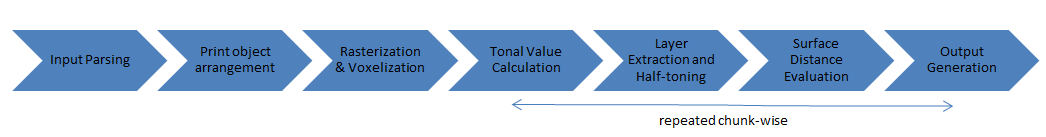
\includegraphics[scale=0.6]{TypicalCuttlefishSteps.PNG}
\caption{Cuttlefish pipeline component functionality}
\label{fig:TypicalCuttlefishSteps}
\end{figure}

\begin{itemize}
\item \textbf{Input Parsing}: The input given to the pipeline, mostly mesh files and textures, is parsed and internal mesh representations are created for them. Internal mesh representations of multiple objects can be grouped together with each having it\textquotesingle s own unique identifier and is known as a print job. At present FileParsePj is the component which performs this task. \newline 

\item \textbf{Print object arrangement}: The print jobs are arranged within the print volume to lower material consumption and print time.The arrangement of the print jobs is done by using a greedy approach where in the print jobs are sorted as per the extent of the bounding box of the print object and best-fit algorithm is applied on the sorted boxes so as to arrange the print objects as compactly as possible in the print volume. PrintJobOrganizer is currently handling this task. \newline 

\item \textbf{Rasterization and Voxelization}: Rasterization is the process of converting an image described in a vector graphics format(shapes) to raster images i.e. pixels or dots for output to the printer or storing it in bitmap format. In voxelization, the mesh representation is converted to voxel representation and each voxel intersecting the surface is assigned attributes like color, occupancy etc. Currently the component doing this is PrintJobVoxelizer. The algorithm used for voxelization can be varied using the component configuration and the description of the voxelization algorithms is beyond the scope of the thesis. \newline 
 
\item \textbf{Tonal Value Calculation}: This step involves calculation and assignment of tonal values from the optical features (RGB or BRDF data) of surface voxels.The tonal value computation is done with the help of a calculated ICC-profile  belonging to the specific printer. The component doing this is called TonalValueCalculator.

\item \textbf{Surface Distance Evaluation and Tonal Analyzer} (optional): The component evaluates the distance of voxels to the surface and assigns values of a given attribute (of the surface voxel)  to inner voxels within the specified mask distance.The Tonal value analyzer component reports summary statistics, comparing the half-toned signal to the original tonal values in easy to interpret graphs.\newline

\item \textbf{Layer Extraction and Half-toning}:It involves extraction of the layers below surface and storing them in a easily accessible way to be used later for halftoning. Half-toning is the process of creating half-tone image. An Half-tone image is comprised of discrete dots rather than continuous tones, when viewed from a distance, the dots blur together, creating the illusion of continuous lines and shapes which helps to save print material. \newline

\item \textbf{Output Generation}: The generated slices are then used to create the desired output i.e. bitmaps or STL files. The output files are then used to drive the print machine. \newline

\end{itemize} 

\section{System Model for distributed Cuttlefish}
 


